%%%%%%%%%%%%%%%%%%%%%%%%%%%%%%%%%
%%  Descrizione dell'architettura
%%%%%%%%%%%%%%%%%%%%%%%%%%%%%%%%%



\subsection{Metodo e formalismo di specifica}
Suddividiamo la descrizione dell'architettura di \proj{} in quattro sezioni:
\begin{itemize}
	\item §\ref{sec:arch_gen}, che illustra gli aspetti generali dell'architettura del software;
	\item §\ref{sec:arch_client}, che descrive l'architettura del \emph{front end} dell'applicazione;
	\item §\ref{sec:arch_server}, che descrive l'architettura del \emph{back end} dell'applicazione;
	\item §\ref{sec:arch_proto}, che descrive il protocollo che lega le due interfacce precedenti.
\end{itemize}
Per ognuna di queste sezioni, procediamo con metodo \emph{top-down} --- dal generale al particolare --- utilizzando i formalismi di UML 2.0.



\subsection{Descrizione generale} \label{sec:arch_gen}
L'architettura dell'applicazione è suddivisa in due moduli:
\begin{enumerate}
	\item il client, che vive nel browser dell'utente;
	\item il server, che fornisce la pagina dell'applicazione al client e riceve da esso delle richieste di generazione di codice.
\end{enumerate}

Tra le varie qualità desiderabili per la nostra architettura, la progettazione ha cercato di perseguire principalmente l'\textbf{estensibilità}. Tale obiettivo è stato raggiunto con due strategie:
\begin{itemize}
	\item in generale, promuovendo le seguenti qualità:
	\begin{itemize}
		\item manutenibilità;
		\item modularità;
		\item semplicità;
		\item basso accoppiamento.
	\end{itemize}
	\item nello specifico, prevedendo le seguenti possibili aggiunte nel futuro:
	\begin{itemize}
		\item Generazione di codice in altri linguaggi target: se i manutentori vorranno generare del codice JavaScript o Python, sarà sufficiente aggiungere dei template per il linguaggio scelto (grazie alla libreria \emph{StringTemplate}).
		\item Diversa compressione del codice generato: attualmente l'applicazione genera un JAR e lo comprime, assieme al file JSON, in formato ZIP; ma si potrebbe facilmente cambiare il formato di compressione in un JAR che contenga egli stesso al suo interno il file JSON.
		\item Persistenza dei dati del diagramma che arrivano in input al \emph{back end}: si potrebbe voler mantenere un database di utenti dell'applicazione, ognuno con i propri diagrammi mantenuti nel server a tempo indefinito; per questo, basta fornire l'indirizzo della risorsa JSON, che attualmente non viene eliminata dal server. % (oppure per ora potremmo eliminarla...)
		\item Persistenza del programma generato: si potrebbe voler mantenere anche il codice generato, come il diagramma di input; per fare ciò, basta garantire al client il carattere persistente della risorsa fornita (badando però a non eliminarla dal server). % (per ora la eliminiamo?)
		\item Diverso formato per i diagrammi in input: si potrebbe voler ricevere dei dati in XML, anziché in JSON; sarà sufficiente modificare il package \texttt{parser}.
	\end{itemize}
\end{itemize}



\subsection{Architettura del client} \label{sec:arch_client}
Il \emph{front end} di \proj{} è una singola pagina web scritta in HTML5, CSS3 e JavaScript.

L'\texttt{head} (intestazione) della pagina HTML contiene dei puntatori a:
\begin{itemize}
	\item le librerie JavaScript elencate nella sezione \ref{sec:tech_client} (con eventuali relativi fogli CSS);
	\item il foglio di stile CSS della pagina;
	\item lo script JavaScript che utilizza le librerie di cui sopra.
\end{itemize}

Il \texttt{body} (corpo) della pagina HTML si compone di pochi blocchi:
\begin{itemize}
	\item dei tag \texttt{div} contenenti i menù laterali da cui selezionare gli strumenti e gli elementi per interagire con i diagrammi;
	\item un tag \texttt{canvas} (identificato dall'\texttt{id} \emph{paper}) che contiene, di volta in volta, il diagramma delle classi o il diagramma di un metodo particolare.
\end{itemize}
Alla ricezione della pagina da parte del client, il nostro script JavaScript popola il tag \texttt{canvas} (inizialmente vuoto) con un diagramma delle classi vuoto.

L'architettura del client è suddivisa in tre package:
\begin{itemize}
	\item \texttt{model}, che gestisce la logica sottostante i diagrammi;
	\item \texttt{view}, che gestisce l'interfaccia grafica;
	\item \texttt{collection}, che raggruppa in una collezione tutti i diagrammi creati.
\end{itemize}

%%% [...]

% >>> RICORDARSI DEL DIAGR. DEI PACKAGE DEL CLIENT 
% \begin{center}
% 	\includegraphics[scale=0.5]{img/pkg_client}
% \end{center}



\subsection{Architettura del server} \label{sec:arch_server}
Il server offre due servizi:
\begin{enumerate}
	\item fornisce al client la pagina HTML dove disegnare i diagrammi;
	\item elabora un file JSON in arrivo dal client e gli fornisce l'applicazione generata a partire da tale file.
\end{enumerate}
Questi due servizi rispettano lo stile architetturale REST (come spiegato più avanti nella sezione \ref{sec:arch_proto}).

Il primo servizio è una semplice pagina HTML, che il server Tomcat gestisce senza nessuna aggiunta da parte nostra.

Il secondo servizio, invece, è una \emph{servlet} Java organizzata nei seguenti package:
\begin{itemize}
	\item \textbf{\texttt{controller}} rappresenta il nucleo del \emph{back end}; un \texttt{RequestHandlerController} si occupa di ricevere ed elaborare le richieste di elaborazione provenienti dal client.
	\item nel package \textbf{\texttt{parser}}, la classe \texttt{Parser} si occupa di convertire il file JSON ricevuto in un oggetto Java di tipo \texttt{ParsedProgram}. Questo oggetto Java rappresenta il programma che l'utente vuole generare; esso si compone di oggetti \texttt{ParsedType} (cioè i tipi definiti dall'utente: gli elementi del diagramma delle classi), i quali si compongono di oggetti \texttt{ParsedAttribute} e \texttt{ParsedMethod}; quest'ultimo tipo si compone a sua volta di oggetti \texttt{ParsedInstruction} e così fia fino ad arrivare alle istruzioni “atomiche”, come ad esempio un \texttt{ParsedReturn}.
	\item \textbf{\texttt{project}} non è altro che il package che organizza i tipi elencati al punto precedente, tutti discendenti da \texttt{ParsedElement}. Inoltre, questo package offre una classe \texttt{ElementFactory}. % che non ho capito cosa fa
	\item \textbf{\texttt{generator}} presenta al suo interno l'interfaccia \texttt{Generator}; le classi che la estendono si occupano di popolare i template \emph{StringTemplate} di un particolare linguaggio di programmazione (\texttt{JavaGenerator} genera codice sorgente Java). % GeneratorAssembler ...
	\item \textbf{\texttt{template}} è il package che organizza i template per linguaggio: dall'interfaccia \texttt{Template} discende, ad esempio, \texttt{JavaTemplate}.
	\item \textbf{\texttt{stereotype}} % boh
	\item \textbf{\texttt{compiler}} presenta l'interfaccia \texttt{Compiler}, le cui implementazioni (specifiche per un certo linguaggio target) compilano il codice sorgente non eseguibile in un programma eseguibile; \texttt{JavaCompiler}, ad esempio, compila codice sorgente Java in \emph{bytecode} per la JVM (Java Virtual Machine) e compatta il codice in un file JAR eseguibile.
	\item \textbf{\texttt{utility}} espone classi di utilità per il programma, come ad esempio una classe \texttt{Compressor} che comprime l'output del compiler in ZIP. % è pulito tenere un package con un nome così generico?
\end{itemize}

% >>> RICORDARSI DEL DIAGR. DEI PACKAGE DEL SERVER 
% \begin{center}
% 	\includegraphics[scale=0.5]{img/pkg_server}
% \end{center}



\subsection{Protocollo di comunicazione client-server} \label{sec:arch_proto}
I due servizi offerti dal server (ottenere la pagina HTML e ottenere l'applicazione generata) seguono lo stile architetturale REST:
\begin{itemize}
	\item La richiesta per ottenere la pagina HTML usa il metodo HTTP GET; la pagina è quindi \emph{cachable} (i router tra client e server possono decidere di ottimizzarne la fornitura).
	\item Il file JSON viene spedito con il metodo HTTP POST, che permette la persistenza di tale file nel server; la persistenza del file JSON è indifferente alla nostra applicazione ma ne aumenta l'estensibilità, in quanto un giorno i manutentori potrebbe voler offrire un servizio di condivisione dei diagrammi disegnati oppure un database di utenti che abbiano i propri diagrammi sul server.
	\item Ognuno dei due servizi (la pagina HTML e la generazione di codice) è una risorsa distinta: questo disaccoppia i due servizi, aumentando ancora la manutenibilità del sistema.
	\item La richiesta per ottenere la pagina HTML è per forza idempotente: lo stato del server non può influire su una pagina statica.
	\item La richiesta di generazione di codice è idempotente: l'unica dipendenza esterna al programma è il file JSON, che viene passato dal client.
\end{itemize}

\begin{center}
	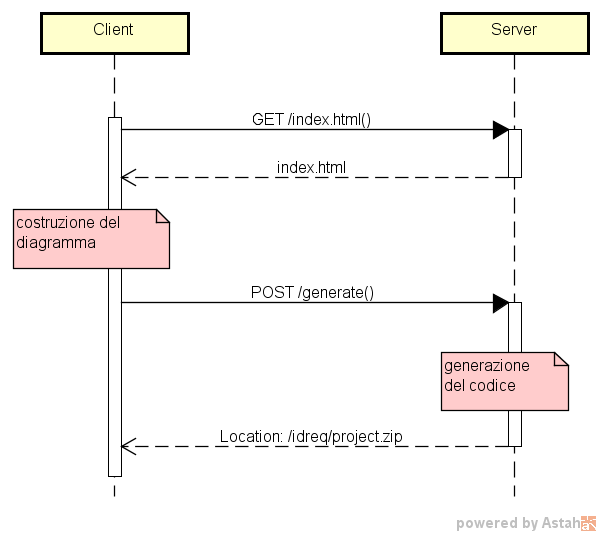
\includegraphics[scale=0.66]{img/http}
\end{center}
